\documentclass[en,11pt]{aghdpl}  % praca w języku angielskim

\usepackage[english]{babel}
\usepackage[utf8]{inputenc}

% dodatkowe pakiety
\usepackage{enumerate}
\usepackage{listings}
\usepackage{verbatim}
\usepackage{booktabs}
\usepackage{mathtools}
\usepackage{textcomp}
\usepackage{amssymb}
\usepackage[table,xcdraw]{xcolor}
\usepackage{siunitx}
\usepackage{hyperref}
\usepackage{float}
\lstloadlanguages{TeX}

\lstset{
  literate={ą}{{\k{a}}}1
           {ć}{{\'c}}1
           {ę}{{\k{e}}}1
           {ó}{{\'o}}1
           {ń}{{\'n}}1
           {ł}{{\l{}}}1
           {ś}{{\'s}}1
           {ź}{{\'z}}1
           {ż}{{\.z}}1
           {Ą}{{\k{A}}}1
           {Ć}{{\'C}}1
           {Ę}{{\k{E}}}1
           {Ó}{{\'O}}1
           {Ń}{{\'N}}1
           {Ł}{{\L{}}}1
           {Ś}{{\'S}}1
           {Ź}{{\'Z}}1
           {Ż}{{\.Z}}1
}

\usepackage{tikz}
\usetikzlibrary{arrows,automata,shapes,positioning,shadows,trees}


%---------------------------------------------------------------------------

\author{Jakub Olesiński}
\shortauthor{J. Olesiński}

\titlePL{Projekt i wykonanie systemu akwizycji i analizy danych dla mobilnej platformy z zespołem dwóch manipulatorów}

\titleEN{Design and development of the system for data acquisition and analysis for the mobile platform with a set of two manipulators.}


\shorttitlePL{Design and development of the system for data acquisition and analysis for the mobile platform with a set of two manipulators.} % skrócona wersja tytułu jeśli jest bardzo długi
\shorttitleEN{Design and development of the system for data acquisition and analysis for the mobile platform with a set of two manipulators.}

%\thesistype{Praca dyplomowa magisterska}
\thesistype{Bachelor of Engineering Thesis}

\supervisor{dr inż. Paweł Rotter}
%\supervisor{Marcin Szpyrka PhD, DSc}

%\degreeprogramme{Automatyka i Robotyka}
\degreeprogramme{Automatics and Robotics}

\date{2013}

%\department{Katedra Automatyki i Inżynierii Biomedycznej}
\department{Department of Automatics and Bioengineering}

%\faculty{Wydział Elektrotechniki, Automatyki,\protect\\[-1mm] Informatyki i Inżynierii Biomedycznej}
\faculty{Faculty of Electrical Engineering, Automatics, Computer Science and Biomedical Engineering}

\acknowledgements{I wish to thank to the Supervisor of this thesis for help and to the ABB Corporate Research Centre for support in the development of this project }


\setlength{\cftsecnumwidth}{10mm}

%---------------------------------------------------------------------------
\setcounter{secnumdepth}{4}

\begin{document}

\titlepages
\setcounter{tocdepth}{3}
\tableofcontents
\clearpage

\chapter*{Introduction}
\markboth{Introduction}{Introduction}
\label{cha:introduction}
\addcontentsline{toc}{chapter}{Introduction}  

%---------------------------------------------------------------------------


The aim of this work is to design and implement a mobile manipulation robotic platform with a vision system for obstacle detection and object recognition with a three dimensional camera. This work is part of a project named "Mobile set of manipulators on a wheeled chassis". The project was realized in a three person team, as part of the Second Edition of ABB Students Scientific Association programme organized by ABB Corporate Research Center in Krakow.

	In the first chapter, a design of the robotic system is presented. General concept of mobile manipulation is outlined with possible application areas. Subsequently, the design requirements, selected hardware components, and implemented software architecture is described. The second chapter provides a survey of modern depth map acquisition techniques, including stereo, time-of-flight and structured light cameras, followed by the selection of a depth sensor. For each method, its operation principle basics and general advantages and disadvantages are provided. The third chapter is focused on modern methods of depth image analysis. An introduction to basic point cloud processing methods is provided, followed by description of a processing tool set for model fitting and object recognition. The final section presents an implementation of the autonomous robot operation mode, based on the 3D image analysis. 
	
	
\begin{comment}

Tematem pracy jest opis wybranych elementów składowych projektu o nazwie: Mobilny zespół manipulatorów na wspólnej platformie jezdnej. Projekt ten zrealizowany został w ramach Drugiej Edycji Koła Naukowego ABB we współpracy z Korporacyjnym Centrum Badawczym ABB w Krakowie. Zespół projektowy składał się z trzech osób pomiędzy które zostały podzielone zadania. Na tej podstawie zrealizowane zostały trzy prace dyplomowe inżynierskie. Niniejsza, związana z projektem mechanicznym, samodzielnym montażem wszystkich podzespołów oraz z analizą zagadnień kinematycznych zespołu dwóch skonstruowanych manipulatorów oraz dwie inne prace związane z oprogramowaniem operatorskim oraz z systemem akwizycji i przetwarzania danych. Projekt był realizowany w okresie od marca do listopada 2014 roku i jego główną częścią było uruchomienie zbudowanego urządzenia i jego prezentacja podczas uroczystego podsumowania.

\end{comment}










\chapter{Mobile manipulation system design}
\label{cha:mmsdesign}

%---------------------------------------------------------------------------

\section{Project background}
\label{sec:background}

A mobile manipulation system (MMS) is a robotic system that is capable of both manipulating objects and locomotion. Typically, the system is composed of a robotic arm based on a robotic mobile platform. Such configuration enables the manipulator to operate in an unlimited workspace, thus providing great application opportunities.

Typically, mobile manipulators are designed to relieve people in hostile situations. They are, for example, widely used in the field of chemical, biological, radioactive or nuclear (CBRN) defense. Explosive materials and other hazardous substances can be disposed without exposing operators to any danger. Another example is space exploration, where manipulation systems are used in planetary rovers in unmanned exploratory missions on other planets. Substitution of human operators in such expeditions significantly reduce their expenditure and risk.

Augmenting the MMS design with a certain degree of autonomy, brings the possibility for the robot to be used as a human-assistant in the household. Most of current applications in this field refer to pick up and delivery services, that have the potential to improve lives of the elderly, injured and disabled people []. Furthermore, typical service robots in human environments are dedicated to accomplish only a single task, such as vacuum cleaning, lawn mowing, pool cleaning or window washing. Their operation is achieved by adjusting existing domestic appliances with a degree of autonomy. With a multi purpose robotic system such as a mobile manipulator, it is potentially possible not to replace existing devices but to substitute the human operator. 

Autonomous gripping and transportation with a MMS could also be used in the industry for designing flexible factory plants and intelligent warehouses []. A manufacturing process that utilizes the MMS robots is simpler and more cost effective in adapting to the market changes. The production could be more customized by applying MMS robots in transportation, preparatory and post-processing tasks. Furthermore, even the most advanced distribution centres, such as the Amazon Kiva Systems [kiva?], require repetitive human work to manipulate goods in the unstructured environment. Therefore, the warehousing process could benefit by applying autonomous MMS robots and there are ongoing efforts in this area [amazonchallenge].

% www.willowgarage.com/pages/pr2/overview

One of the most promising applications of MMS is the PR2 development platform from the Willow Garage company. PR2 is a human-sized robot, equipped with two 7 degree-of-freedom manipulators, omnidirectional mobile base, a processing power of two Xeon servers with 8 cores and 24GB of RAM each, and a multitude of sensors, including stereo, time-of flight and structured light cameras, LIDAR scanners, and an inertial measurement unit [prspecs]. The PR2 robot has already proven successful in such dexterous experiments as opening doors, playing pool, folding towels and serving beverages to people[prapps]. 

Wide functionality of a MMS robot makes its design a challenging task. In MMS robots, the unstructured environment and additional degrees of freedom complicate the control task. Furthermore, the workspace of a manipulator is often shared with people and other vehicles. Such work environment renders many potentially hazardous situations. Therefore, it requires a highly sophisticated control system, with vision based feedback. 

%---------------------------------------------------------------------------

\section{Design requirements}
\label{sec:require}

Design requirements:
\begin{enumerate}
\item The robotic system should consist of two cooperating serial manipulators, based on a wheeled robotic platform.
\item The whole construction should be made of easily accessible components, preferably available on the consumer market, as it would ease the maintenance of the equipment in the future.
\item Both serial manipulators should be equiped with grippers for general object manipulation.
\item Their reachable workspace should allow to reach objects located on the ground.
\item The workspace of each manipulator should also intersect, to allow collaboration on manipulation tasks.
\item The steering mechanisms of the MMS chassis should be kept simple and convenient to control.
\item The platform is expected to move only on flat surfaces at indoor areas.
\item The MMS robot should possess a control server, that is expected to provide a web interface, developed in a commonly used and well supported standard.
\item That interface is required to provide methods for setting positions on manipulator joints, for setting speed of achieving those positions, and for setting velocity and direction of platform movement. 
\item Processing power of the computing unit should be sufficient to analyse camera images in an online fashion. 
\item The whole system should be powered by a source that could withstand at least an hour of continuous work.
\end{enumerate}

\begin{comment}
In robotics a serial manipulator is a device used to manipulate objects. It consists of a kinematic chain with actuated joints. The type of the joint can be prismatic or revolute, correspondingly allowing for either rotational or transational motion. The last link of the chain is called an end-effector, which is used to interact with the environment.
 
 
 Robotic arm reachable workspace is defined as a set of points at which end-effector can be located. Manipulators are usually classified by their structural configuration, that is, the type of first three joints in the kinematic chain. We distignuish four basic types of such configuration: 

\begin{enumerate}
\item Cartesian - three prismatic joints \textcolor{red}{pros/cons}
\item Cylindrical - two prismatic and one revolute joints \textcolor{red}{pros/cons}
\item Spherical - one prismatic and two revolute joints  \textcolor{red}{pros/cons}
\item Articulated - three revolute joints  \textcolor{red}{often called antromorphic, since it mimics human arm structure. It provides relatively large workspace and is convinient for obstacle avoidance, although it is the most difficult in positioning. }
\end{enumerate}

 For every manipulator, the position and orientation of its end-effector can be derived from its joint positions and its geometric model. The inverse problem however, is more difficult and does not always have a solution. In 1968 Donald L. Peiper showed that \textit{the inverse kinematics of serial manipulators with six revolute joints, and with three consecutive joints intersecting, can be solved in closed-form, i.e. analytically}. This result is referred to as \textcolor{red}{321 kinematic structure []}, since the three wrist joints intersect, the two shoulder and elbow joints are parallel, and the first joint orthogonally intersects the first shoulder joint. The 321 design is an example of a 6R wrist-partitioned manipulator, which is one the most widely used type of manipulator in the industry.
 
 Modern industrial robotic arms are characterized with high precision and repeatability. They usually work in a fixed workspace, on factory plants, where they relieve humans from repeatable, dull and often dangerous tasks.\textcolor{red}{ On the other hand, limited workspace of a manipulator imposes high costs of any changes in the manufacturing process. Inflexibility of the plant to different products [].}


Generally speaking, a mobile robotic platform is an automatic machine that is capable of locomotion. Movement of a robot can be achieved in various ways, such as walking, rolling, hopping, metachronal motion etc. In general, wheeled robots consume less energy than other locomotion mechanisms. [1] The most crucial aspect of design in such robots is the type of used wheel. Standard wheels, although simple in structure and good in reliability, impose nonholonomic velocity constraints that limit robot motion. On the other hand, there are special wheel designs, with which a robot can obtain omnidirectional motion, removing those constraints. Mecanum wheels are an example of such wheels. They were invented in 1973 by Bengt Ilon, an engineer in Swedish company Mecanum AB [2]. In principle, they are composed of a central wheel with a set of rollers attached on its periphery at a certain angle. Depending on each individual wheels direction and speed, the total force vector can be achieved in any desired direction, ensuring three degrees of freedom for planar motion of the whole platform. [3]


A mobile manipulator is a robotic system composed of a mobile platform and a robotic arm. Combining locomotion with manipulation enables the manipulator to operate in unlimited workspace, which makes it more flexible and provides great application possibilities. On the other hand, such design considerably complicates the control task. Due to additional degrees of freedom and unstructured environment, additional systems need to be introduced. A robot of that kind requires simultaneous navigation, path planning, object recognition and manipulation. Workspace of a mobile manipulator is usually shared with people and other vehicles, which render many potentially hazardous situations and impose entirely new and high demands on the security system. Addressing those problems have already been widely discussed in the literature, for example in [8][9][10].

Mobile manipulation requires a data acquisition system with a variety of sensors to collect information about the environment and accomplish its tasks. Navigational information for dead reckoning task is usually gathered by odometry sensors, inertial units, and sometimes by RF position-location systems. Typically, tactile bumpers and ultrasonic or infrared proximity sensors provide necessary data to solve collision avoidance problems. Stereo-cameras, time-of-flight cameras, laser LIDARs and RGB-D sensors are generally utilised in vision systems resolving tasks such as object recognition and pose estimation. A vision system that provides depth information can also serve as a collision avoidance system or may navigate the robot.

%---------

The MPTM robot consists of two robotic arms based on a simple four-wheeled mobile platform. Both of robotic arms have 5 degrees of freedom and are in articulated structural configuration. To avoid complicating the mechanical design of the chassis with a steering mechanism, a special kind of wheels were used. Mecanum wheels, as they are called, are equipped with a set of rollers attached to their circumference, which allow a vehicle to move in any direction without turning the wheels. 

By alternating wheels with left and right-handed rollers, in such a way that each wheel applies force roughly at right angles to the wheelbase diagonal the wheel is on, the vehicle is stable and can be made to move in any direction and turn by varying the speed and direction of rotation of each wheel. Moving all four wheels in the same direction causes forward or backward movement, running the wheels on one side in the opposite direction to those on the other side causes rotation of the vehicle, and running the wheels on one diagonal in the opposite direction to those on the other diagonal causes sideways movement. Combinations of these wheel motions allow for vehicle motion in any direction with any vehicle rotation.

Another advantage of such design is increased stability of the platform.

The MPTM robot utilises two types of actuators, 4 DC motors for the mobile platform wheels and 12 servomechanisms for manipulator joints. 
All DC motors have 50:1 metal gearboxes. They achieve 200 RPM of no-load speed and 12 kg cm of stall current. Additionally, they possess 64 CPR encoders, which multiplied by the gear ratio provide 3200 counts per revolution.

Servomechanisms used are Turnigy 1269HV, with operating speed of 

Actuators are driven by PWM signal generated by MSP430G2553 microcontrollers, one for each of manipulators and one for the mobile platform.

%---------------------------------------------------------------------------

Mobile manipulators have been widely used in research and non-industrial applications, such as human assistance, planetary exploration or CBRN defense. 

Typical service robots in human environments are specially designed to accomplish only a single task, such as vacuum cleaning, lawn mowing, pool cleaning, window washing etc. Their operation is achieved by adjusting existing domestic apliances with a degree of autonomy. With a multi purpose robotic system such as a mobile manipulator, it is potentially possible not to replace existing devices but to replace the operator. Most of the actual applications refer to pick up and delivery services, which have the potential to improve the lives of elderly, injured and disabled, as discussed in []. One of the most successful applications is the PR2 robot from Willow Garage company. The PR2 is being programmed to do increasingly technical and dexterous applications including opening doors and folding towels. [][]

More often, mobile manipulators are designed to relieve people in hostile situations. They are, for example, widely used in the field of chemical, biological, radioactive or nuclear (CBRN) defense. Bombs and other hazardous substances can be disposed without exposing operators to any danger. Another example is space exploration, where manipulation systems are used in planetary rovers in unmanned exploratory missions on other planets. Substitution of human operators in such expeditions significantly reduce their expenditure and risk. In both situations, used robotic systems have to be characterized by high reliability and must be prepared to withstand unknown surface. While CBRN defense robots are usually radio controlled due to the highly complicated manipulation tasks, planetary rovers lack that privilige. Long delays. Recent Curiosity rover was capable of ...

Exploration - the other hand, high demands, reasons, recent Curiosity

CBRN defense, widely used, reasons, demands, example

Industry - conservative, environment can be known, all required technology exists, flexible factories.

\end{comment}


%---------------------------------------------------------------------------

\section{Hardware components}
\label{sec:hard}

Mechanical structure:

\begin{figure}[H]
\centering
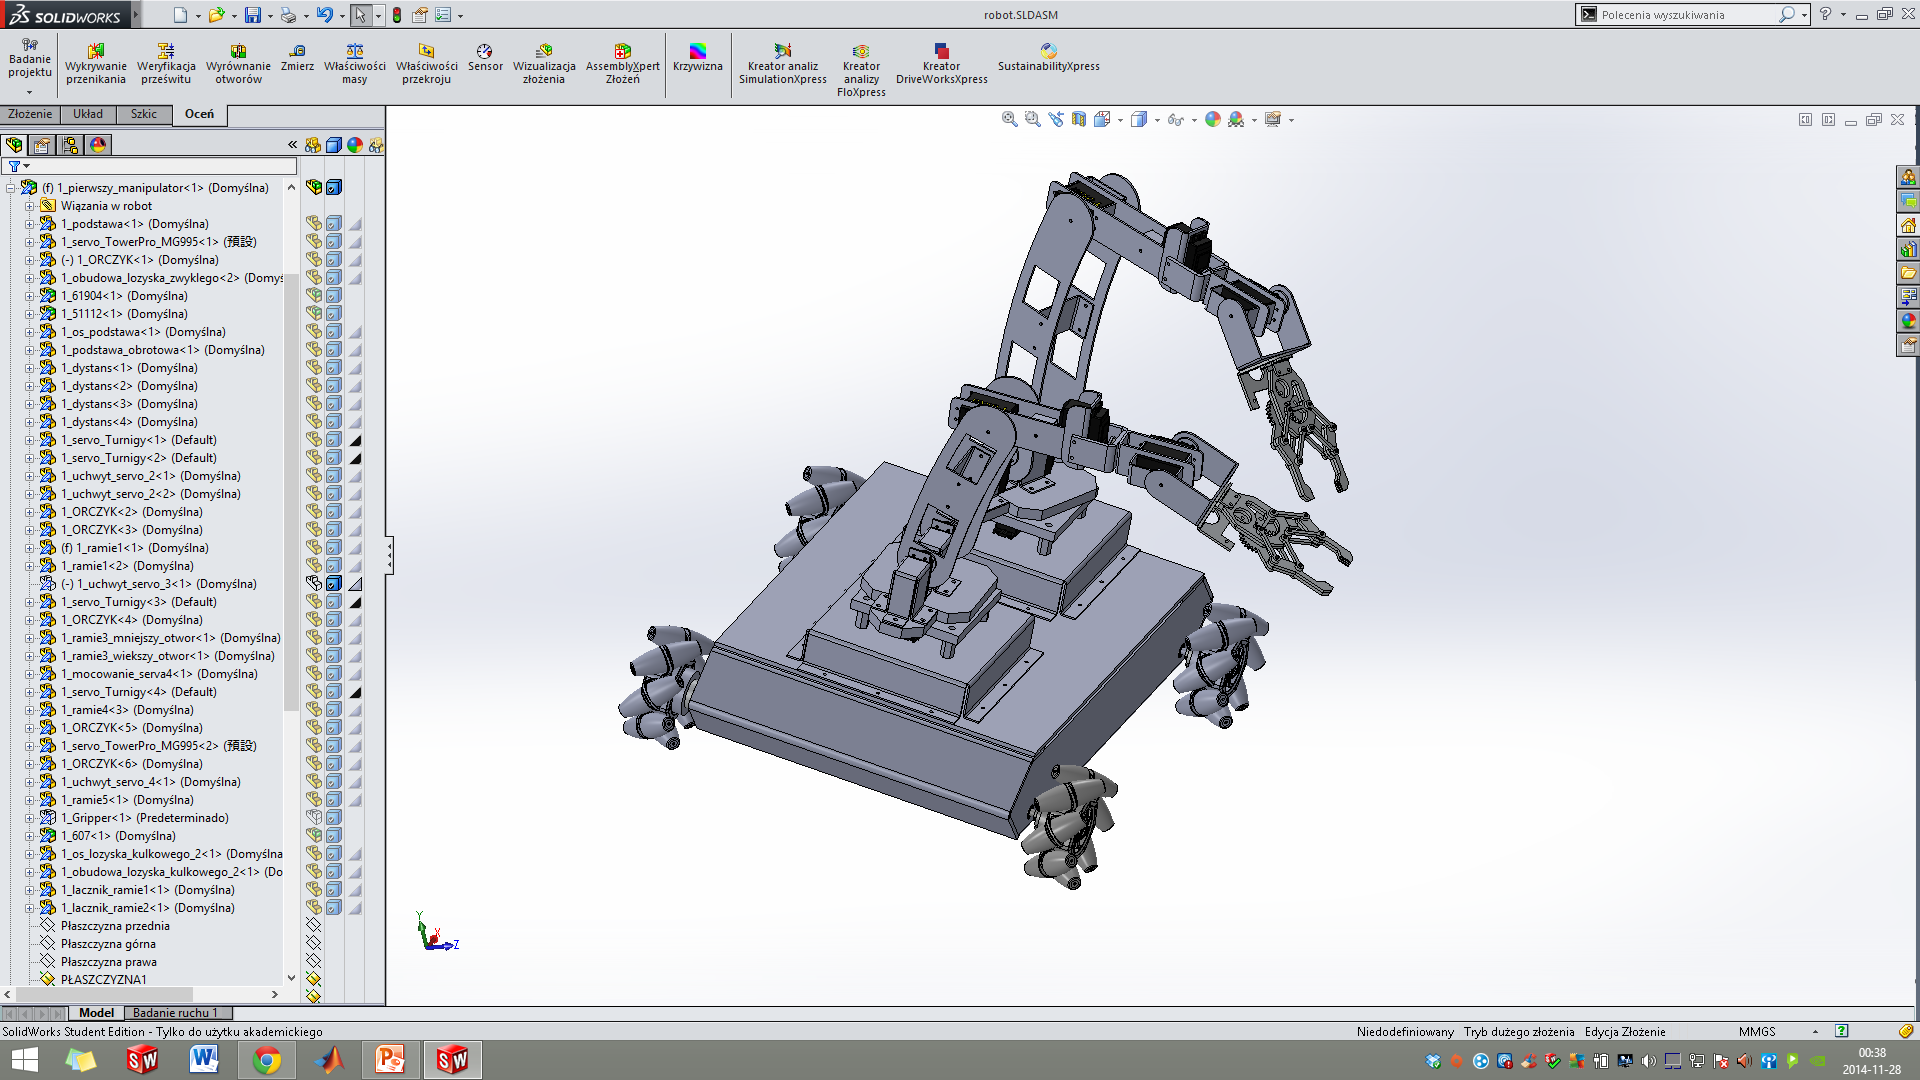
\includegraphics[trim=21cm 5cm 18cm 5cm, clip=true, totalheight=0.5\textheight]{fig/model}
\caption{Model}
\end{figure}

The MPTM robot consists of two robotic arms based on a simple four-wheeled mobile platform. Both of robotic arms have 5 degrees of freedom and are in articulated structural configuration. To avoid complicating the mechanical design of the chassis with a steering mechanism, a special kind of wheels were used. Mecanum wheels, as they are called, are equipped with a set of rollers attached to their circumference, which allow a vehicle to move in any direction without turning the wheels. 

By alternating wheels with left and right-handed rollers, in such a way that each wheel applies force roughly at right angles to the wheelbase diagonal the wheel is on, the vehicle is stable and can be made to move in any direction and turn by varying the speed and direction of rotation of each wheel. Moving all four wheels in the same direction causes forward or backward movement, running the wheels on one side in the opposite direction to those on the other side causes rotation of the vehicle, and running the wheels on one diagonal in the opposite direction to those on the other diagonal causes sideways movement. Combinations of these wheel motions allow for vehicle motion in any direction with any vehicle rotation.

Another advantage of such design is increased stability of the platform.

Basic components:

\tikzset{
  basic/.style  = {draw, drop shadow, font=\sffamily, font=\footnotesize, rectangle,text centered, minimum size=2.2cm,minimum height=0.5cm},
  root/.style   = {basic, thin, align=center, fill=blue!25},
  level 2/.style = {basic, thin,align=center, fill=blue!30},
  level 3/.style = {basic, thin, align=center, fill=blue!35}
}
\begin{figure}[H]
\centering
\begin{tikzpicture}[
  level 1/.style={sibling distance=30mm},
  edge from parent/.style={->,draw},
  >=latex]

% root of the the initial tree, level 1
\node[root] {Hardware\\Components}
% The first level, as children of the initial tree
  child {node[level 2] (c1) {Mobile platform}}
  child {node[level 2] (c2) {Two robotic arms}}
  child {node[level 2] (c3) {CPU}}
  child {node[level 2] (c4) {Power}}
  child {node[level 2] (c5) {Peripherals}};

% The second level, relatively positioned nodes
\begin{scope}[every node/.style={level 3}]
\node [below of = c1, xshift=15pt] (c11) {DC Motors\\ Pololu 50:1 6V};
\node [below of = c11] (c12) {Mecanum wheels};
\node [below of = c12] (c13) {Motor controller\\ Rover V};

\node [below of = c2, xshift=15pt] (c21) {Servomotors \\ Turnigy 1269HV};
\node [below of = c21] (c22) {End-effectors};
\node [below of = c22] (c23) {Servo controller\\ PCA9685};

\node [below of = c3, xshift=15pt] (c31) {Raspberry Pi};
\node [below of = c31] (c32) {NVidia Jetson};


\node [below of = c4, xshift=15pt] (c41) {Li-Poly battery \\ 8S 5.8Ah};
\node [below of = c41] (c42) {DC-DC converter};


\node [below of = c5, xshift=15pt] (c51) {Asus Xtion sensor};
\end{scope}

% lines from each level 1 node to every one of its "children"
\foreach \value in {1,2,3}
  \draw[->] (c1.195) |- (c1\value.west);

\foreach \value in {1,...,3}
  \draw[->] (c2.195) |- (c2\value.west);

\foreach \value in {1,...,2}
  \draw[->] (c3.195) |- (c3\value.west);
  
\foreach \value in {1,...,2}
  \draw[->] (c4.195) |- (c4\value.west);
  
\foreach \value in {1,...,1}
  \draw[->] (c5.195) |- (c5\value.west);
\end{tikzpicture}

\caption{Components}
\end{figure}

The MPTM robot utilises two types of actuators, 4 DC motors for the mobile platform wheels and 12 servomechanisms for manipulator joints. 
All DC motors have 50:1 metal gearboxes. They achieve 200 RPM of no-load speed and 12 kg cm of stall current. Additionally, they possess 64 CPR encoders, which multiplied by the gear ratio provide 3200 counts per revolution.

Servomechanisms used are Turnigy 1269HV, with operating speed of 

Actuators are driven by PWM signal generated by MSP430G2553 microcontrollers, one for each of manipulators and one for the mobile platform.

End effect:


\begin{figure}[H]
\centering
\includegraphics[trim=15cm 18cm 28cm 10cm, clip=true, totalheight=0.4\textheight]{fig/robot}
\caption{Construction}
\end{figure}
%---------------------------------------------------------------------------

\section{Software architecture}
\label{sec:soft}

%http://www.texample.net/tikz/examples/data-flow-diagram/
\begin{figure}[H]
\begin{center}
\begin{tikzpicture}
  [auto,every node/.style={rectangle,draw,align=center, font=\footnotesize}]
  
  \node (manual) at (1,10) {Manual controller \\ (Android, PC)};
  \node[below right=of manual] (raspberry) {Control Server \\ (Raspberry Pi)};
  \node[below left=of raspberry] (auto) {Autonomous mode \\ (NVIDIA Jetson TK1)};
  \node[above right=of raspberry] (servo) {Servocontroller \\ (PCA9685)};
  \node[below right=of raspberry] (motor) {Motor controller \\ (Rover 5)};
  %\node[draw=none,fill=none, node distance=2mm, above=of match1](ann1) {\small Recognition Pipeline for Local Descriptors};

  % draw the paths and and print some Text below/above the graph
 \path (manual.east) 	edge[bend left=20]  node[anchor=south,above]{$SC_n=0$}
                                    node[anchor=north,below]{$RN_{16}$} (raspberry.west)
(auto.east) 	edge[bend left=20]  node[anchor=south,above]{$SC_n=0$}
                                    node[anchor=north,below]{$RN_{16}$} (raspberry.west)
 (raspberry.east)     	edge[bend right=20] node[anchor=south,above]{$SC_n\neq 0$} (motor.west)
 (raspberry.east)  	edge[bend right=20] node[anchor=left,right]{$SC_n = 0$} (servo);



  %\foreach \from/\to in {manual/raspberry,auto/raspberry,raspberry/servo,raspberry/motor}
   % \draw[->] (\from) -- (\to);

\end{tikzpicture}

\caption{Software architecture}

\label{fig:softdesign}

\end{center}
\end{figure}

\chapter{Depth data acquisition techniques}
\label{cha:acquisition}

\begin{comment}
[1] - Build Your Own 3D Scanner

What is a depth map. Classification of aqcuisition methods - passive and active, number of vantage points. This chapter provides a brief description of the operating principle of some commonly used techniques with their advantages and disadvantages.
\end{comment}


The manipulation and movement tasks of a MMS robot involves continuous interaction with unstructured and changing environment. In order to develop an autonomous system, which will be able to operate in such conditions, a data acquisition system is required, that would provide the necessary information about the nearby objects surface, size and relative distances. The measurement of this type can be performed by using depth acquisition techniques, also known as three dimensional (3D) imaging.

The first depth acquisition techniques emerged as a replacement for a contact-based coordinate measuring machines (CMM). CMMs were used in the industrial quality control applications and worked by recording the displacement of a probe tip sliding across a solid surface. Such method was time consuming and inadequate for fragile objects. Modern, contact-less 3D scanning apparatus overcome those limitations by using light to interact with the environment. The new technology has also extended the application area of 3D scanning to the field of robotic perception.

Modern methods of 3D data acquisition are classified by the light source they utilize to measure depth. \textit{Passive} techniques rely only on the ambient light, whereas the \textit{active} ones operate by projecting illumination onto an object and recording the reflected beam. In the following sections, examples of both categories are presented, with a brief description of their principles of operation and a discussion of advantages and disadvantages, finalized by hardware selection for the designed MMS robot.

%-------------------------------------------------------

\section{Stereo vision}
\label{sec:stereo}

\begin{comment}
[1] - State-Of-The-Art and Applications of 3D imaging sensors
Pic: http://zone.ni.com/reference/en-XX/help/372916M-01/nivisionconceptsdita/guid-cb42607e-f256-40f5-ab6e-28ec3a33bcda/

Passive method. Based on human vision - biological process of Stereopsis. Depth info acquired using two or more images concurrently captured from displaced cameras. Processing steps: image acquisition, camera modeling, feature extractions, correspondence analysis and triangulation. Simple, low-cost hardware, but processing computationally expensive. Features? Correspondences? Triangulation with picture.

\end{comment}

Stereo vision is a passive depth acquisition technique, widely used in research and  industry. Its principle of operation is based on human vision system and the biological process of stereopsis, where the disparity between two different projections of the world on the human retinas leads to the depth sensation. Analogically, in computer stereo vision technique, two (or more) displaced in space cameras concurrently acquire the scene view. From the captured images disparity, a scene depth information is then inferred. A typical scheme for stereo vision depth calculation after image acquisition is divided into two steps: the correspondence problem and triangulation.

The correspondence problem is the most difficult part of the stereo vision. It can be stated as follows: given two displaced 2D images of the same scene, find points representing the same space location in those images. There are many point matching algorithms discussed in the literature. Some of them rely on computing point features, based on their neighbourhood, while others compute statistical descriptors of characteristic areas in the image, and then minimise the measured difference between analysed regions to find the best matches. The correspondence problem in computer vision is a wide and open research area, that is beyond the scope of this work. A thorough description of the problem and its solutions, is provided, for example, by \cite{Cyganek}.

\begin{figure}[H]
\label{fig:stereo}
\centering
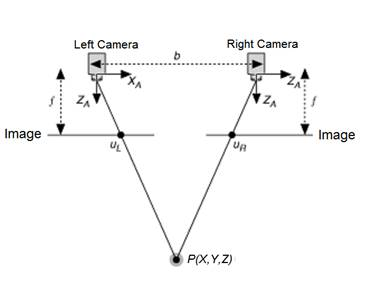
\includegraphics[width=0.5\textwidth]{fig/nistereovision}
\caption{A simplified stereo vision system \cite{nistereo}}
\label{fig:stereovision}
\end{figure}


After obtaining the corresponding points, the point depth information can be derived by the means of triangulation (Figure \ref{fig:stereovision}). if the imaging properties of the camera are known, two three-dimensional lines, from the camera's projection centres to the examined point can be drawn. The intersection of those lines is then used to infer the depth of the point. 

The main advantage of the stereo vision system is that it can be built with easily accessible, standard 2D cameras. Such cameras allow to reduce the expenditure and provide relatively high resolution. On the other hand, the stereo vision systems have many drawbacks. Firstly, their performance is reduced in environments with low ambient light intensity, which makes the system impractical in some settings. Secondly, the depth accuracy decreases quadratically with the distance. Finally, the algorithms used for feature extraction and matching, involved in solving the correspondence problem are computationally expensive and often limit the depth acquisition frame rate.


 There also exists a variant of active stereo vision, utilized i.e. in the Ensenso N10 cameras \cite{ensenso}. In this case, besides the camera pair, a pattern projector is applied to add artificial texture to the scene, which helps to determine the disparity on untextured surfaces.



\begin{comment}
WIKIPEDIA:

Computer stereo vision is the extraction of 3D information from digital images, such as obtained by a CCD camera. By comparing information about a scene from two vantage points, 3D information can be extracted by examination of the relative positions of objects in the two panels. This is similar to the biological process Stereopsis.

\begin{figure}[H]
\centering
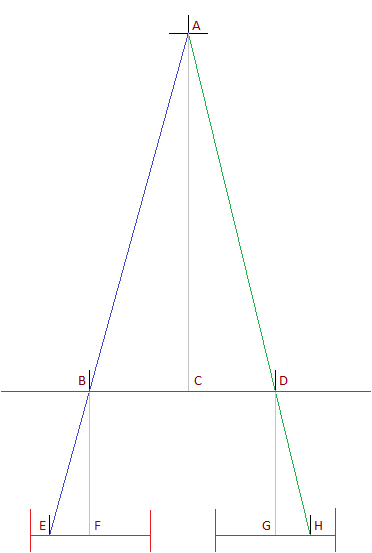
\includegraphics[scale=0.7]{stereo}
\caption{Stereo vision}
\end{figure}

In traditional stereo vision, two cameras, displaced horizontally from one another are used to obtain two differing views on a scene, in a manner similar to human binocular vision. By comparing these two images, the relative depth information can be obtained, in the form of disparities, which are inversely proportional to the differences in distance to the objects.

To compare the images, the two views must be superimposed in a stereoscopic device, the image from the right camera being shown to the observer's right eye and from the left one to the left eye.

In real camera systems however, several pre-processing steps are required.

The image must first be removed of distortions, such as barrel distortion to ensure that the observed image is purely projectional.
The image must be projected back to a common plane to allow comparison of the image pairs, known as image rectification.
An information measure which compares the two images is minimized. This gives the best estimate of the position of features in the two images, and creates a disparity map.
Optionally, the disparity as observed by the common projection, is converted back to the height map by inversion. Utilising the correct proportionality constant, the height map can be calibrated to provide exact distances.
%---------------------------------------------------------------------------
\end{comment}


\begin{comment}
%\section{Laser LIDAR}
%\label{sec:lidar}

WIKIPEDIA:


Lidar (also written LIDAR or LiDAR) is a remote sensing technology that measures distance by illuminating a target with a laser and analyzing the reflected light. Although thought by some to be an acronym of Light Detection And Ranging, the term lidar was actually created as a portmanteau of "light" and "radar."

Lidar is popularly used as a technology to make high-resolution maps, with applications in geomatics, archaeology, geography, geology, geomorphology, seismology, forestry, remote sensing, atmospheric physics, airborne laser swath mapping (ALSM), laser altimetry, and contour mapping.

Lidar uses ultraviolet, visible, or near infrared light to image objects. It can target a wide range of materials, including non-metallic objects, rocks, rain, chemical compounds, aerosols, clouds and even single molecules.[4] A narrow laser-beam can map physical features with very high resolution[vague].

Lidar has been used extensively for atmospheric research and meteorology. Lidar instruments fitted to aircraft and satellites carry out surveying and mapping – a recent example being the U.S. Geological Survey Experimental Advanced Airborne Research Lidar.[12] NASA has identified lidar as a key technology for enabling autonomous precision safe landing of future robotic and crewed lunar-landing vehicles.[13]

Wavelengths vary to suit the target: from about 10 micrometers to the UV (approximately 250 nm). Typically light is reflected via backscattering. Different types of scattering are used for different lidar applications: most commonly Rayleigh scattering, Mie scattering, Raman scattering, and fluorescence. Based on different kinds of backscattering, the lidar can be accordingly called Rayleigh Lidar, Mie Lidar, Raman Lidar, Na/Fe/K Fluorescence Lidar, and so on.[4] Suitable combinations of wavelengths can allow for remote mapping of atmospheric contents by identifying wavelength-dependent changes in the intensity of the returned signal.

\end{comment}
%---------------------------------------------------------------------------

\section{Time of flight}
\label{sec:tof}

\begin{comment}
http://www.ti.com/lit/wp/sloa190b/sloa190b.pdf
\end{comment}

Time of flight (ToF) cameras work on a completely different principle than stereoscopic systems. ToF systems are characterised with active illumination and are composed of an near infra-red (IR) emmiter and IR camera. They work by illuminating the scene with a modulated IR beam and recording the received light, as presented in the figure 5. The distance from the recorded object is then calculated by measuring the phase shift between the illuminated and reflected signals. 

In the simplest form, the ToF cameras use single light pulses \cite{titof}. After a short period of illumination, the reflected energy is then integrated at every pixel with two out of phase windows over the same $\Delta t$ time, resulting in two electrical charges $Q_1$ and $Q_2$. The depth distance $d$ is then computed as $d = \frac{1}{2}c\Delta t \frac{Q_2}{Q_1+Q_2}$, where $c$ is the speed of light constant. A more advanced method is to project illumination modulated by a continuous wave signal, commonly a square wave. In this case, four sampling windows, shifted by \SI{90}{\degree} angle, resulting in $Q_1$,$Q_2$, $Q_3$ and $Q_4$ charges. The phase angle $\phi$ between the projected and the reflected signals is given by $\phi = arctan \frac{Q_3 - Q_4}{Q_1 - Q_2} $ and the final depth $d = \frac{c}{4\pi f}\phi$. The principle of the continuous wave method is illustrated by the Figure \ref{fig:tofprinciple}.

ToF cameras, due to their specific architecture, are prone to errors caused by radiometric, geometric and illumination variations. The power of the emitted IR signal limits their measurement accuracy. The light entering to the sensor has an ambient and reflected components, thus high ambient light intensity reduces the signal to noise ratio. Moreover, the material and color of the object surface cause variations in the amplitude of the reflected IR signal.

\begin{figure}[H]
\label{fig:tof}
\centering
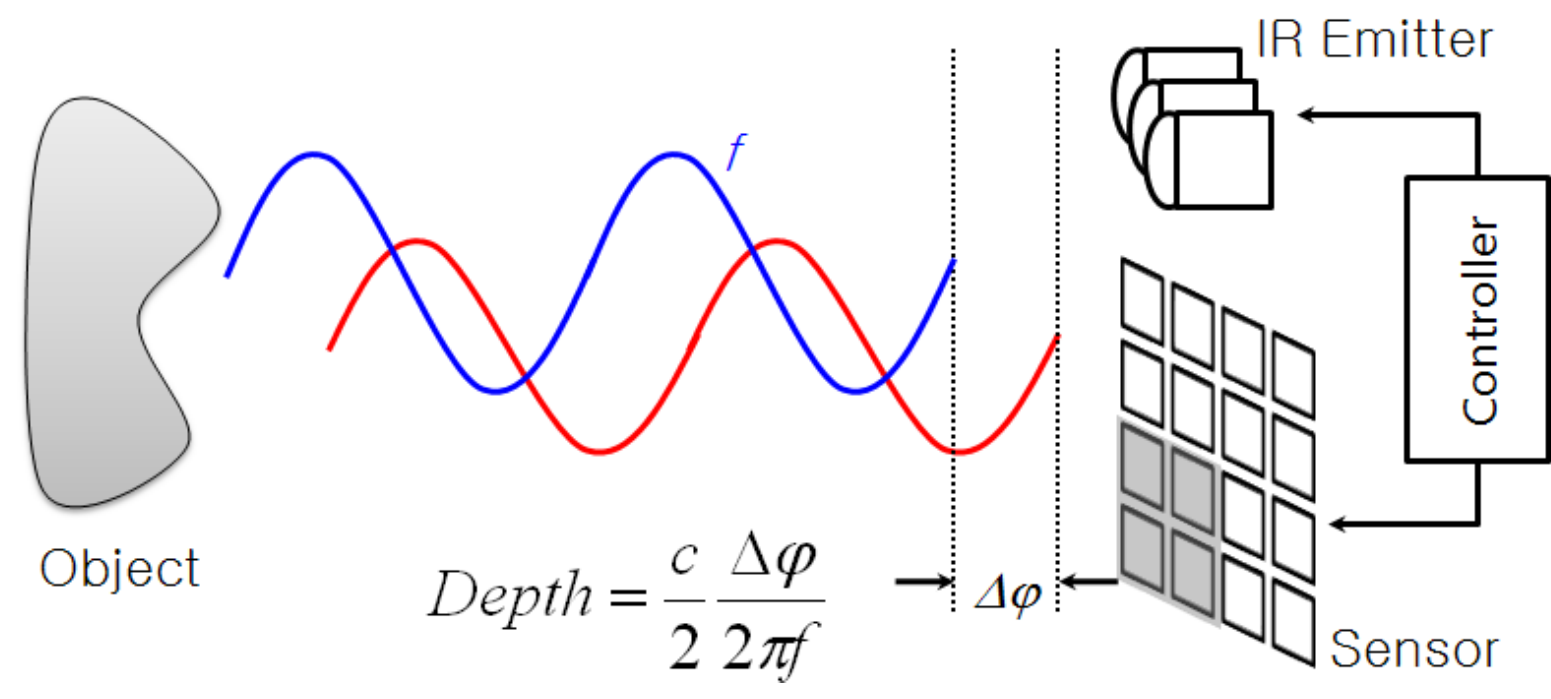
\includegraphics[width=0.7\textwidth]{fig/tofprinciple}
\caption{Time of flight with continuous wave modulation \cite{ToFbook}}
\label{fig:tofprinciple}
\end{figure}

Despite problems arising from ToF principle of operation, modern ToF cameras are distinguished by relatively low latency and fast scanning speed. The depth measurements are acquired directly from the hardware, so the speed is not limited by software processing. Unfortunately, most of the products available on the end-user market provide relatively low depth image resolution, typically QQVGA (160x120) and the price increases significantly with the resolution.


\begin{comment}
WIKIPEDIA:


A time-of-flight camera (ToF camera) is a range imaging camera system that resolves distance based on the known speed of light, measuring the time-of-flight of a light signal between the camera and the subject for each point of the image. The time-of-flight camera is a class of scannerless LIDAR, in which the entire scene is captured with each laser or light pulse, as opposed to point-by-point with a laser beam such as in scanning LIDAR systems.[1]

The simplest version of a time-of-flight camera uses light pulses or a single light pulse. The illumination is switched on for a very short time, the resulting light pulse illuminates the scene and is reflected by the objects in the field of view. The camera lens gathers the reflected light and images it onto the sensor or focal plane array. Depending upon the distance, the incoming light experiences a delay. As light has a speed of approximately c = 300,000,000 meters per second, this delay is very short: an object 2.5 m away will delay the light by 16 ns.

The single pixel consists of a photo sensitive element (e.g. a photo diode). It converts the incoming light into a current. In analog timing imagers, connected to the photo diode are fast switches, which direct the current to one of two (or several) memory elements (e.g. a capacitor) that act as summation elements. In digital timing imagers, a time counter, that can be running at several gigahertz, is connected to each photodetector pixel and stops counting when light is sensed.

Advantages:

Simplicity
In contrast to stereo vision or triangulation systems, the whole system is very compact: the illumination is placed just next to the lens, whereas the other systems need a certain minimum base line. In contrast to laser scanning systems, no mechanical moving parts are needed.

Efficient distance algorithm
It is a direct process to extract the distance information out of the output signals of the TOF sensor. As a result, this task uses only a small amount of processing power, again in contrast to stereo vision, where complex correlation algorithms are implemented. After the distance data has been extracted, object detection, for example, is also a straightforward process to carry out because the algorithms are not disturbed by patterns on the object.

Speed
Time-of-flight cameras are able to measure the distances within a complete scene with a singleshot. As the cameras reach up to 160 frames per second, they are ideally suited to be used in real-time applications.

Disadvantages:

Background light
When using CMOS or other integrating detectors or sensors that use visible or near visible light (400 nm - 700 nm), although most of the background light coming from artificial lighting or the sun is suppressed, the pixel still has to provide a high dynamic range. The background light also generates electrons, which have to be stored. For example, the illumination units in many of today's TOF cameras can provide an illumination level of about 1 watt. The Sun has an illumination power of about 50 watts per square meter after the optical band-pass filter. Therefore, if the illuminated scene has a size of 1 square meter, the light from the sun is 50 times stronger than the modulated signal. For non-integrating TOF sensors that do not integrate light over time and are using near-infrared detectors (InGaAs) to capture the short laser pulse, direct viewing of the sun is a non-issue because the image is not integrated over time, rather captured within a short acquisition cycle typically less than 1 microsecond. Such TOF sensors are used in space applications[19] and in consideration for automotive applications.[24]

Interference
In certain types of TOF devices, if several time-of-flight cameras are running at the same time, the TOF cameras may disturb each other's measurements. To be clear, this is not true of all TOF sensors. There exist several possibilities for dealing with this problem:

Time multiplexing: A control system starts the measurement of the individual cameras consecutively, so that only one illumination unit is active at a time.
Different modulation frequencies: If the cameras modulate their light with different modulation frequencies, their light is collected in the other systems only as background illumination but does not disturb the distance measurement.
For Direct TOF type cameras that use a single laser pulse for illumination, because the single laser pulse is short (e.g. 10 nano-seconds), the round trip TOF to and from the objects in the field of view is correspondingly short (e.g. 100 meters = 660nS TOF round trip), for an imager capturing at 30 Hz, the probability of an interfering interaction is the time that the camera acquisition gate is open divided by the time between laser pulses or approximately 1 in 50,000 (0.66uS divided by 33mS).

Multiple reflections
In contrast to laser scanning systems where a single point is illuminated, the time-of-flight cameras illuminate a whole scene. For a phase difference device (amplitude modulated array), due to multiple reflections, the light may reach the objects along several paths. Therefore, the measured distance may be greater than the true distance. Direct TOF imagers are vulnerable if the light is reflecting from a specular surface. There are published papers available that outline the strengths and weaknesses of the various TOF devices and approaches.

\end{comment}

%---------------------------------------------------------------------------

\section{Structured light}
\label{sec:actuators}

The structured light (SL) depth measurement technique combines some of the features of both time of flight and stereo vision principles.  Similarly to ToF cameras, SL relies on active illumination, work in the near infra-red and is composed of an IR emitter and IR camera. As in the case of stereo vision, depth information is inferred from the disparity between two images by the means of triangulation. In this case, the projected IR pattern is compared with the image captured by the IR camera. The IR projector emits patterns of non-coherent light, which then appears distorted from the perspective of the camera. In such settings, the projection of defined patterns makes explicit correspondences on the reflected image. A typical setting of the SL system is presented in figure 5.


%http://www.extremetech.com/extreme/131159-leap-motion-will-it-make-you-a-magician-or-is-it-just-handwaving
\begin{figure}[H]
\label{fig:sl}
\centering
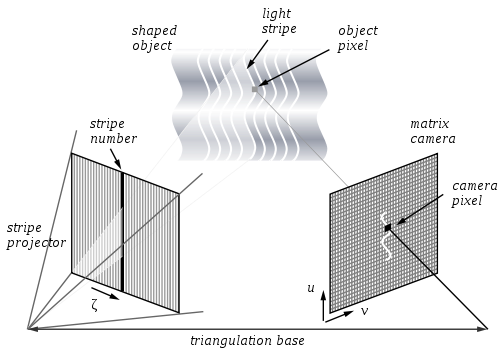
\includegraphics[width=0.6\textwidth]{fig/structuredlight}
\caption{Structured light fringe patterns \cite{extremetech}}
\label{fig:slprinciple}
\end{figure}

	There are many pattern strategies that allow for correspondence identification, including projections of grids, dots, vertical slits and multi-color patterns. In the literature, particular attention is paid to fringe patterns (Figure \ref{fig:slprinciple}), which are suitable to maximize the measurement resolution \cite{sensors}. Moreover, to reduce the reconstruction artifacts, the measurement process is often extended into a sequence of different pattern projections. A comprehensive assessment of such pattern codes can be found in \cite{slcodes}.
	
	Depth measuring devices that employ the SL technique suffer from many drawbacks. Utilizing multiple pattern frames introduces high latency and makes the measurement ill conditioned for dynamic scenes. Moreover, the system performance is degraded in bright ambient light. On the other hand, popular SL devices are characterized with relatively high, VGA (640x480) depth map resolution and are easily accessible on the consumer market.


	A particularly noteworthy application of SL based depth data acquisition device is the Kinect by Microsoft. In addition to an RGB camera and an array of microphones, the device includes an IR projector-camera pair from the PrimeSense Ltd. company, used for depth measurements. The SL light pattern used in Kinect is a non-periodic speckle pattern produced by the interference of partially coherent beams (Figure X). In this device, every pixel is identified in the IR image using a correlation window, after which the depth information is calculated, using triangulation. The Kinect device is produced as a gaming controller for the Xbox 360 console and it is widely available at the consumer market with a relatively low price. Moreover, there are many open source drivers for the Kinect device, which make it a perfect match for robotic and research applications.
	
\begin{figure}[H]
\centering
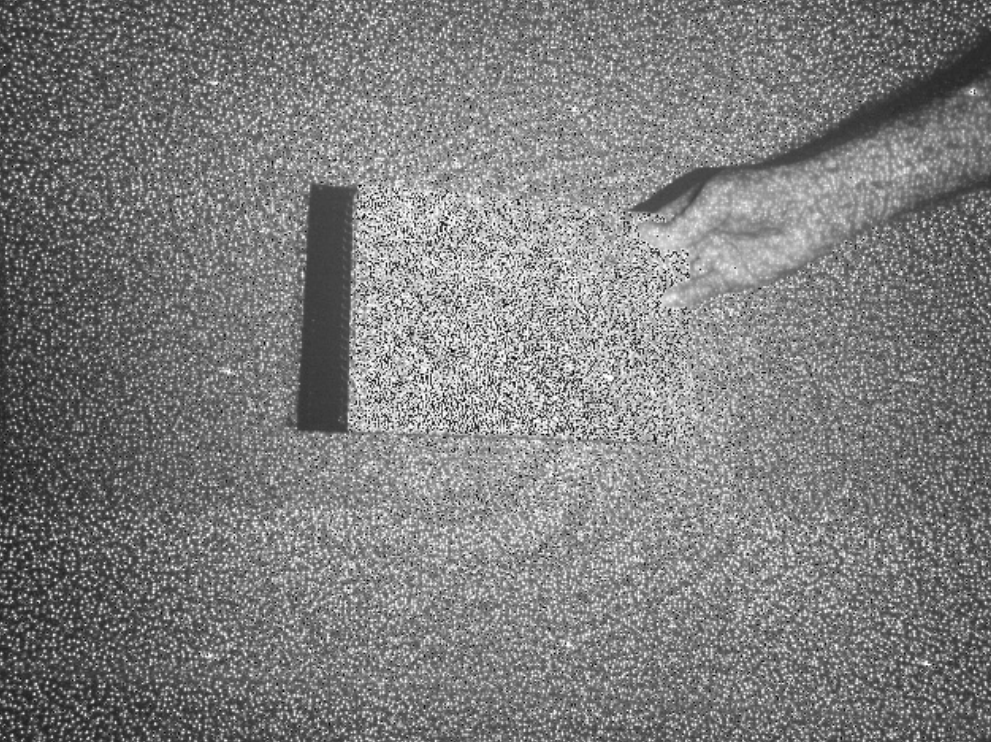
\includegraphics[scale=0.25]{fig/KinectSpeckle}
\caption{Kinect speckle pattern \cite{borenstein2012making}}
\label{fig:kinectspeckle}
\end{figure}
	


\begin{comment}

WIKIPEDIA:


Projecting a narrow band of light onto a three-dimensionally shaped surface produces a line of illumination that appears distorted from other perspectives than that of the projector, and can be used for an exact geometric reconstruction of the surface shape (light section).

A faster and more versatile method is the projection of patterns consisting of many stripes at once, or of arbitrary fringes, as this allows for the acquisition of a multitude of samples simultaneously. Seen from different viewpoints, the pattern appears geometrically distorted due to the surface shape of the object.

Although many other variants of structured light projection are possible, patterns of parallel stripes are widely used. The picture shows the geometrical deformation of a single stripe projected onto a simple 3D surface. The displacement of the stripes allows for an exact retrieval of the 3D coordinates of any details on the object's surface.



Two major methods of stripe pattern generation have been established: Laser interference and projection.

The laser interference method works with two wide planar laser beam fronts. Their interference results in regular, equidistant line patterns. Different pattern sizes can be obtained by changing the angle between these beams. The method allows for the exact and easy generation of very fine patterns with unlimited depth of field. Disadvantages are high cost of implementation, difficulties providing the ideal beam geometry, and laser typical effects like speckle noise and the possible self interference with beam parts reflected from objects. Typically, there is no means of modulating individual stripes, such as with Gray codes.

The projection method uses non coherent light and basically works like a video projector. Patterns are generated by a display within the projector, typically a liquid crystal display (LCD) or liquid crystal on silicon (LCOS) display.

A proprietary projection method uses digital light processing (DLP; moving micro mirror) displays. DLP displays do not absorb light significantly and therefore allow very high light intensities. They also have an extremely linear gray value reproduction, as they are steered by pulse length modulation.

Principally, stripes generated by display projectors have small discontinuities due to the pixel boundaries in the displays. Sufficiently small boundaries however can practically be neglected as they are evened out by the slightest defocus.

A typical measuring assembly consists of one stripe projector and at least one camera. For many applications, two cameras on opposite sides of the projector have been established as useful.

Invisible (or imperceptible) structured light uses structured light without interfering with other computer vision tasks for which the projected pattern will be confusing. Example methods include the use of infrared light or of extremely high framerates alternating between two exact opposite patterns.[2]

There are several depth cues contained in the observed stripe patterns. The displacement of any single stripe can directly be converted into 3D coordinates. For this purpose, the individual stripe has to be identified, which can for example be accomplished by tracing or counting stripes (pattern recognition method). Another common method projects alternating stripe patterns, resulting in binary Gray code sequences identifying the number of each individual stripe hitting the object. An important depth cue also results from the varying stripe widths along the object surface. Stripe width is a function of the steepness of a surface part, i.e. the first derivative of the elevation. Stripe frequency and phase deliver similar cues and can be analyzed by a Fourier transform. Finally, the wavelet transform has recently been discussed for the same purpose.

In many practical implementations, series of measurements combining pattern recognition, Gray codes and Fourier transform are obtained for a complete and unambiguous reconstruction of shapes.

Another method also belonging to the area of fringe projection has been demonstrated, utilizing the depth of field of the camera.[3]

It is also possible to use projected patterns primarily as a means of structure insertion into scenes, for an essentially photogrammetric acquisition.


\end{comment}


\section{Summary and hardware selection}
\label{sec:3dsum}

%http://www.ti.com/ww/en/analog/3dtof/index.shtml?DCMP=hpa_contributed_article&HQS=3dtof-ca

Three of the most popular depth map acquisition techniques were presented in this chapter, including stereo vision, time of flight and structured light. Each method has its advantages and disadvantages and they all have already been successfully applied in robotics. A comparative summary of each method characteristics is presented in Table \ref{tab:depthcompar}.

\begin{table}[h]
\begin{center}
\begin{tabular}{@{}rccc@{}}
\toprule
Feature/Technique                                                                                            & Stereo Vision                                                                                                   & Time of Flight                                                                                                       & Structured Light \\ \midrule
\rowcolor[HTML]{EFEFEF} 
\multicolumn{1}{r|}{\cellcolor[HTML]{EFEFEF}\begin{tabular}[c]{@{}r@{}}Depth data\\ generation\end{tabular}} & \multicolumn{1}{c|}{\cellcolor[HTML]{EFEFEF}\begin{tabular}[c]{@{}c@{}}Directly out \\ of chipset\end{tabular}} & \multicolumn{1}{c|}{\cellcolor[HTML]{EFEFEF}\begin{tabular}[c]{@{}c@{}}High software\\ processing\end{tabular}}      & \begin{tabular}[c]{@{}c@{}}Medium software\\ processing\end{tabular}      \\
\multicolumn{1}{r|}{Latency}                                                                                 & \multicolumn{1}{c|}{Medium}                                                                                     & \multicolumn{1}{c|}{Low}                                                                                             & Medium                                                                    \\
\rowcolor[HTML]{EFEFEF} 
\multicolumn{1}{r|}{\cellcolor[HTML]{EFEFEF}\begin{tabular}[c]{@{}r@{}}Low light\\ performance\end{tabular}} & \multicolumn{1}{c|}{\cellcolor[HTML]{EFEFEF}Weak}                                                               & \multicolumn{1}{c|}{\cellcolor[HTML]{EFEFEF}Good}                                                                    & Good                                                                      \\
\multicolumn{1}{r|}{\begin{tabular}[c]{@{}r@{}}Bright light\\ performance\end{tabular}}                      & \multicolumn{1}{c|}{Good}                                                                                       & \multicolumn{1}{c|}{Medium}                                                                                          & Medium                                                                    \\
\rowcolor[HTML]{EFEFEF} 
\multicolumn{1}{r|}{\cellcolor[HTML]{EFEFEF}\begin{tabular}[c]{@{}r@{}}Power\\ consumption\end{tabular}}     & \multicolumn{1}{c|}{\cellcolor[HTML]{EFEFEF}Low}                                                                & \multicolumn{1}{c|}{\cellcolor[HTML]{EFEFEF}\begin{tabular}[c]{@{}c@{}}Medium - scales\\ with distance\end{tabular}} & \begin{tabular}[c]{@{}c@{}}Medium - scales \\ with distance\end{tabular}  \\
\multicolumn{1}{r|}{Resolution}                                                                              & \multicolumn{1}{c|}{Camera dependent}                                                                           & \multicolumn{1}{c|}{QQVGA, QVGA}                                                                                     & VGA, 1080p                                                                \\
\rowcolor[HTML]{EFEFEF} 
\multicolumn{1}{r|}{\cellcolor[HTML]{EFEFEF}Accurracy}                                                       & \multicolumn{1}{c|}{\cellcolor[HTML]{EFEFEF}mm, cm}                                                              & \multicolumn{1}{c|}{\cellcolor[HTML]{EFEFEF}mm, cm}                                                                  & \SI{}{\micro\meter}, cm                                                                    \\
\multicolumn{1}{r|}{Scanning speed}                                                                          & \multicolumn{1}{c|}{\begin{tabular}[c]{@{}c@{}}Medium - limited by\\  software complexity\end{tabular}}         & \multicolumn{1}{c|}{\begin{tabular}[c]{@{}c@{}}Fast - limited by \\ sensor speed\end{tabular}}                       & \begin{tabular}[c]{@{}c@{}}Fast - limited by\\  camera speed\end{tabular} \\ \bottomrule
\end{tabular}
\caption {Qualitative comparison of depth acquisition techniques \cite{titof}}

\label{tab:depthcompar}
% 2 - http://www.ti.com/ww/en/analog/3dtof/index.shtml?DCMP=hpa_contributed_article&HQS=3dtof-ca
\end{center}
\end{table}

In order to fulfil project assumptions, one solution providing depth map measurement had to be chosen. In the stereo vision technology, ready-made devices unfortunately did not fit within the project budget. Utilizing this technique would therefore require an own design of the stereo vision system. Such solution would probably be the least expensive, but require an extensive amount of work and time. Therefore, the author focused on finding a ready-made solution in the remaining technologies. The DepthSense 311 [3] device was found as a representative of the ToF technique, and the Asus Xtion Pro Live [4] was considered as an option from the SL method. Both devices are available in similiar prices and provide the same frame rate of 30 frames per second. The Asus device, however, offers higher depth map resolution (VGA instead of QQVGA) and has better support from the open source community. The Asus Xtion is based on the PrimeSense Ltd. depth sensing hardware, similarly to the popular Kinect device and is even compatible with the same open source drivers. Nonetheless, it was chosen over the Kinect device, because it has smaller size and is powered directly from the USB port (the Kinect requires external power source). Main specifications of the Asus Xtion Pro device are provided in the Table \ref{tab:asus}.

\begin{table}[h]

\begin{center}

\begin{tabular}{r||l}
\hline
Operating range      & Between 0.8m and 3.5m                                                                   \\

\hline
Field of view        & \SI{58}{\degree H}, \SI{45}{\degree V}, \SI{70}{\degree D} \\

\hline
Depth map resolution & \begin{tabular}[c]{@{}l@{}}VGA (640x480) : 30 fps\\ QVGA (320x240): 60 fps\end{tabular} \\

\hline
Interface            & USB2.0/ 3.0                                                                             \\

\hline
Dimensions           &  18 x 3.5 x 5 cm  \\ \hline
\end{tabular}
\caption{Asus Xtion Pro Live specification \cite{ASUS}}
\label{tab:asus}
\end{center}
\end{table}

\chapter{Analysis of the depth data}
\label{cha:analysis}

The acquired depth information can be stored in computer memory in two ways. The first is the depth map, which takes the form of a two dimensional array, similarly to the plain gray-scale image. In this case, however, the depth measurement is stored in place of the color intensity. Depth map is the simplest way to represent and store the acquired depth of the scene and it is usually obtained directly from the sensor driver. The main disadvantage of a depth map is its inflexibility. This representation is strictly bound to the camera point of view and thus it is inconvenient in further processing.

The second representation of a scene's depth information is a point cloud. Generally speaking, it is a set of data points in some coordinate system. Typically, the Cartesian system is used and the points are defined by their x, y and z coordinates. Point clouds are derived from depth maps and offer new capabilities, such as viewpoint transformation or cloud concatenation.

 Furthermore, most software libraries provide an interface to interactively manipulate and visualize the point cloud, which is a useful tool when 

This chapter presents the main tools used further in the implementation of the autonomous control mode for the MMS robot.

%---------------------------------------------------------------------------

\section{Basic point cloud processing}
\label{sec:pointclouds}

A frequently used operation during the processing of a point cloud is the affine transformation. Point clouds can be translated, rotated and scaled by multiplying a transformation matrix $A \in \mathbb{R}^{4x4}$ with data points in homogeneous coordinates $[x,y,z,1]^T$. Basic transformation matrices are presented in the Figure \ref{fig:transformations}. Presented transformations can be further composed by multiplication to produce more complex ones.

\begin{figure}[H]  

  \begin{minipage}{.3\linewidth}
    \centering
    \[A_t=\left[\begin{array}{cccc}
      1 & 0 & 0 & t_x \\
      0 & 1 & 0 & t_y \\
      0 & 0 & 1 & t_z \\
      0 & 0 & 0 & 1
    \end{array}\right]\]
    Translation by a vector $t=[t_x,t_y,t_z]^T$
  \end{minipage}%
  \begin{minipage}{.3\linewidth}
    \centering
    \[A_s=\left[\begin{array}{cccc}
      S_x & 0 & 0 & 0 \\
      0 & S_y & 0 & 0 \\
      0 & 0 & S_z & 0 \\
      0 & 0 & 0 & 1
    \end{array}\right]\]
    Scaling along $x,y,z$ by factors $S_x,S_y,S_z$
  \end{minipage}  
  \begin{minipage}{.4\linewidth}
    \centering
    \[A_x=\left[\begin{array}{cccc}
      1 & 0 & 0 & 0 \\
      0 & cos(\theta_x) & -sin(\theta_x) & 0 \\
      0 & sin(\theta_x) & cos(\theta_x) & 0 \\
      0 & 0 & 0 & 1
    \end{array}\right]\]
    Rotation around $x$ with \\ $\theta_x$ angle
  \end{minipage}%
  
  \begin{minipage}{.5\linewidth}
    \centering
    \[A_y=\left[\begin{array}{cccc}
      cos(\theta_y) & 0 & sin(\theta_y) & 0 \\
      0 & 1 & 0 & 0 \\
      -sin(\theta_y) & 0 & cos(\theta_y) & 0 \\
      0 & 0 & 0 & 1
    \end{array}\right]\]
    Rotation around $y$ with $\theta_y$ angle 
  \end{minipage}
  \begin{minipage}{.5\linewidth}
    \centering
    \[A_z=\left[\begin{array}{cccc}
      cos(\theta_z) & -sin(\theta_z) & 0 & 0 \\
      sin(\theta_z) & cos(\theta_z) & 0 & 0 \\
      0 & 0 & 1 & 0 \\
      0 & 0 & 0 & 1
    \end{array}\right]\]
    Rotation around $z$ with $\theta_z$ angle 
  \end{minipage}
  
  
  \caption{Basic affine transformations}
  \label{fig:transformations}
\end{figure}

%Info from pcl tutorials.

Preprocessing. Another useful type of operation is spatial filtering. Probably the most basic filter is the pass-through filter, which reject all points outside a given range along a specified dimension. This procedure allows to focus the analysis process on the region of interest, i.e. the reachable workspace of a manipulator. Apart from limiting the cloud dimensions, the number of data points can be also reduced by downsampling. The voxel grid filter is typically used for this purpose. This filter creates a three dimensional regular grid over the input point cloud data and then, in each voxel, approximates all the present data points with their centroid. Such reduction is particularly useful when large point cloud datasets have to be processed online with limited computing resources. Finally, the filtration process has to cope with numerous measurement errors present in the raw data acquired from the 3D camera. Such measurement noise 
manifests itself in the form of sparse outliers, which corrupt the results of further processing, i.e. the surface normals estimation. The impact of those irregularities can by reduced by applying an outlier removal filter. The simplest form of such filter rejects all the data points which does not have enough neighbours within a specified radius. A more refined version is based on the neighbouring points distance distribution. Firstly, the mean distance from each point to all its neighbours is calculated. Next, based on the assumption that the resulting distribution is Gaussian, all the points whose mean distances lay outside of an interval defined by the global distances mean and their standard deviation are rejected from the dataset. The effects of statistical outlier removal are presented in the Figure 222.


\begin{figure}[H]
\label{fig:outlierremoval}
\centering
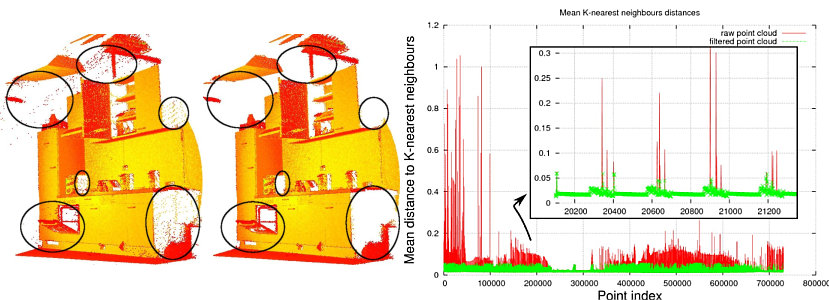
\includegraphics[width=0.9\textwidth]{fig/statistical_removal}
\caption{Statistical outlier removal [tutorials]}
\end{figure}

%Info from Rusu dissertation

In a given point cloud, a single point by itself does not provide much information about the surface to analyse. Therefore, an essential concept in depth data analysis is the local neighbourhood of a point. For a query point $p_q$ in the point cloud $P$ its neighbourhood is given by:
\begin{equation}
d(p_	q, p_i) \leq r
\end{equation}
where $p_i \in P$ is the neighbouring point, $d$ is the selected metric, typically Euclidean, and $r>0$ is the neighbourhood radius. In practice, approximate methods are used, as direct application would require calculation of distance from the query point $p_q$ to all other points in $P$. The algorithms used for neighbourhood search require a parameter $k$ specifying the maximum number of points in the neighbourhood or parameter $r$, denoting the maximum search radius. Proper determination of those parameters is crucial in further analysis. Too small values will not provide enough information about the surface. Too large, on the other hand, will average the surface and skip small details.



Many of the algorithms used further during the analysis of a point cloud base on the notion of a surface normal, known from the 3D geometry. These vectors are also widely used for shading in 3D computer graphics and a variety of methods have already been developed to solve the surface normal estimation problem. One of the simplest uses the least-squares plane fitting to estimate the normal to a plane tangent to the surface, which approximates the desired vector [Rusu]. More specifically, for a given point on the surface, it's $k$-neighbourhood centroid $\bar{p}$ is calculated as:
\begin{equation} 
\bar{p} = \frac{1}{k} \cdot \sum\limits_{i=1}^{k} p_i 
\end{equation}
The tangent plane is thereafter defined by the centroid $\bar{p}$ and the sought normal vector $\vec{n}$. The latter is computed by minimizing the total (squared?) distance from every k-neighbour $p_i$ to the tangent plane, given by $\sum\limits_{i=1}^{k} (p_i - \bar{p})\cdot \vec{n}$. The minimization problem can be solved by utilizing the covariance matrix $C \in \mathbb{R}^{3x3}$, given by:
\begin{equation}
C = \frac{1}{k}\sum\limits_{i=1}^{k}(p_i - \bar{p})\cdot (p_i - \bar{p})^\intercal
\end{equation}
The covariance matrix $C$ is symmetric, positive semi-definite and possess three real eigenvalues $\lambda_j \geq 0, i = 1,2,3$. The eigenvector corresponding to the smallest eigenvalue is an approximation of the desired normal vector $\vec{n}$, disregarding the sign. Furthermore, if the viewpoint $v_p$ is known, the normal $\vec{n}$ has to be oriented towards  $v_p$, which means that it has to satisfy the equation:
\begin{equation}
\vec{n}\cdot(v_p-p_i) > 0
\end{equation}


%---------------------------------------------------------------------------

\section{The Random Sample Consensus algorithm}
\label{sec:ransac}
The indoor human environment is abundant of regularly shaped objects that could be described with basic geometrical models, such as planes, spheres or cylinders. The plane model:
\begin{equation}
\theta_1 \cdot x+\theta_2 \cdot y+\theta_3 \cdot z+\theta_4 = 0
\end{equation}
is particularly useful, as the floor, walls or furniture is typically composed of flat surfaces. By knowing which points belong to the surface of a floor, the robot can autonomously navigate and avoid collisions. For this reason, a robust model fitting algorithm is a strongly desired tool in the analysis of the depth data. The point dataset received from the depth camera , however, consists of both points that belong to the model, the inliers, and a lot of other points in the scene, the outliers. Therefore direct usage of classic model fitting algorithms, such as the least squares method, would not provide the desired effect, as they try to fit the model into all the input data points, including outliers. As an alternative, the Random Sample Consensus (RANSAC) algorithm, can effectively cope with such problems. In its basic form, the RANSAC algorithm is essentially composed of two, iteratively repeated steps [Dummies,Wiki]:
\begin{enumerate}
\item Firstly, a minimal sample subset is randomly selected from the input dataset. The model parameters are computed using only the selected subset. The cardinality of the subset is the smallest sufficient to determine the model parameters.
\item Secondly, the remaining dataset points are tested to be consistent with the model computed in the sampling step. A data point will be considered as an inlier if it fits the computed model within a defined error threshold. The set of such elements is called a consensus set. If the consensus set contains enough points, the model is reestimated from all selected inliers and evaluated with the error of the inliers relative to the model.
\end{enumerate}
This procedure is then repeated until a termination condition is met, which usually is a fixed number of iterations.
The main advantage of the RANSAC algorithm is the robust estimation. This method is able to fit a model with high accuracy even if the data set contains a significant amount of outliers. On the other hand, the algorithm in its basic form has several disadvantages. There is no upper bound on the time needed to estimate model parameters and by limiting the number of iterations, the obtained solution is may not be optimal. Furthermore, the RANSAC algorithm can only estimate one model per dataset and if multiple models exist, it may fail to estimate any of them. Since the original RANSAC was first published in 1981, it has been widely adapted by the image processing community and many modifications that address the RANSAC limitations has been proposed. A comparative summary of the recent extensions to the RANSAC algorithm can be found for example in [dunno].

%---------------------------------------------------------------------------

\section{Descriptors for object recognition}
\label{sec:descriptors}

Descriptors what for. Difference between global and local. Itemize some global and local with brief description. Table with comparison. Reference to detailed info.

Object recognition - problem formulation. Point cloud matching etc.

Surface normals are the most basic representation of the geometry around a certain point. Even if coupled with surface curvature, they usually does not provide enough descriptive information for object recognition and pose estimation. To achieve better performance in such tasks, more complex and higher dimensional descriptors have been proposed in the literature [summary]. A descriptor is considered to be good if it is able to capture the same surface characteristics, regardless of rigid transformations, varying sampling density and noise. In general, 3D shape descriptors a divided into local and global. The former describe only the local geometry around a query point, while the latter represent the geometry of a whole object. A few selected descriptors will be presented further in this section.

The Point Feature Histogram (PFH) is a generalization of both surface normals and curvature estimates. It represents the relative orientation of normals between every point pair $(p_i,p_j)$ in the neighbourhood of the query point $p_q$. For each point pair, using the surface normal $n_i$ at $p_i$, a new coordinate frame $u,v,w$ is constructed as follows:
\begin{equation}
u = n_i,\  v = u \times \frac{p_i-p_j}{d},\  w = u \times v
\end{equation}
where $d = \|p_i-p_j\|_2$ is the Euclidean distance between $p_i$ and $p_j$. Using this reference frame, the difference between normals at $p_i$ and $p_j$ is expressed by the angular features $\alpha, \phi, \theta$, given by:
\begin{equation}
\label{eq:angularfeat}
\alpha = v \cdot n_i, \  \phi = u \cdot \frac{(p_i-p_j)}{d}, \ \theta = arctan(w\cdot n_i, u \cdot n_i)
\end{equation}
Finally, to create the PFH descriptor, the angular features are binned into a histogram. The angular ranges are typically divided into 5 subdivisions, thus receiving a $3^5=125$ binned histogram, that counts occurrences of any value combination for every point pair $(p_i, p_j)$.

The main disadvantage of the PFH descriptor is its $O(nk^2)$ complexity, where $n$ is the number of points in the point cloud and $k$ is the number of each points neighbours. For large datasets, this is one of the major bottlenecks during online processing. To overcome this problem a simplification to the PFH formulation, called Fast Point Feature Histogram has been proposed (FPFH) [Proposal]. In the first step of the FPFH, the angular features $\alpha, \phi, \theta$ are computed only between the query point $p_q$ and its k-nearest neighbours, as described in Equation \ref{eq:angularfeat}. Those features produce a histogram, called Simplified Point Feature Histogram (SPFH). 	The SPFH is computed for every point in the cloud, and then, the FPFH descriptor is formed as follows:
\begin{equation}
FPFH(p_q) = SPFH(p_q) + \frac{1}{k}\sum\limits_{i=1}^k\frac{1}{w_i}SPFH(i)
\end{equation}
where $w_i$ is a distance between $p_q$ and $p_k$ in some metric space. The FPFH descriptor reduces the computational complexity of the PFH to $O(nk)$, while maintaining similar descriptive performance.

Figure: Influence diagrams

SHOT or VFH

%PFH, FPFH, SHOT,	Keypoint extraction, VFH

%---------------------------------------------------------------------------

\section{The Iterative Closest Point algorithm}
\label{sec:icp}

%---------------------------------------------------------------------------

\section{Object recognition pipeline}
\label{sec:pipeline}

\begin{figure}[H]
\begin{center}
\begin{tikzpicture}
  [node distance = 5mm,auto,every node/.style={rectangle,draw,align=center, font=\footnotesize}]
  
  \node (kpextr) at (1,10) {Key Point \\ Extraction};
  \node[right=of kpextr] (descr1) {Description};
  \node[right=of descr1] (match1) {Matching};
  \node[draw=none,fill=none, node distance=2mm, above=of match1](ann1) {\small Recognition Pipeline for Local Descriptors};
  \node[right=of match1] (corr) {Correspondence \\ Grouping};
  \node[right=of corr] (absor) {Absolute \\ Orientation};
  \node[below right=of absor] (icp) {ICP \\ Refinement};
  \node[right=of icp] (verify) {Hypothesis \\ Verification};
  \node[below left=of icp] (align) {Alignment};
  \node[left=of align] (match2) {Matching};
  \node[left=of match2] (descr2) {Desription};
  \node[left=of descr2] (segm) {Segmentation};
  \node[draw=none,fill=none, node distance=2cm, below=of ann1](ann2) {\small Recognition Pipeline for Global Descriptors};


  \foreach \from/\to in {kpextr/descr1,descr1/match1, match1/corr, corr/absor, absor/icp, icp/verify, segm/descr2, descr2/match2, match2/align, align/icp}
    \draw[->] (\from) -- (\to);

\end{tikzpicture}

\caption{Object recognition pipeline [IEEE]}

\label{fig:objpipe}

\end{center}
\end{figure}

\chapter{Implementation and testing}
\label{cha:implandtest}

%---------------------------------------------------------------------------

\section{Algorithm implementation}
\label{sec:implementatnion}


%---------------------------------------------------------------------------

\section{Testing in the real environment}
\label{sec:testing}


\chapter*{Summary}
\label{cha:summary}
\addcontentsline{toc}{chapter}{Summary}  

%---------------------------------------------------------------------------

%\section{Testing}
%\label{sec:testing}


%---------------------------------------------------------------------------

%\section{Conclusions}
%\label{sec:conclusions}


%---------------------------------------------------------------------------

%\section{Future development}
%\label{sec:future}







% itd.
% \appendix
% \include{dodatekA}
% \include{dodatekB}
% itd.

\bibliographystyle{ieeetr}
\bibliography{bibliografia}
%\begin{thebibliography}{1}
%
%\bibitem{Dil00}
%A.~Diller.
%\newblock {\em LaTeX wiersz po wierszu}.
%\newblock Wydawnictwo Helion, Gliwice, 2000.
%
%\bibitem{Lam92}
%L.~Lamport.
%\newblock {\em LaTeX system przygotowywania dokumentów}.
%\newblock Wydawnictwo Ariel, Krakow, 1992.
%
%\bibitem{Alvis2011}
%M.~Szpyrka.
%\newblock {\em {On Line Alvis Manual}}.
%\newblock AGH University of Science and Technology, 2011.cccccc
%\newblock \\\texttt{http://fm.ia.agh.edu.pl/alvis:manual}.
%
%\end{thebibliography}

\end{document}
